\documentclass[1p]{elsarticle_modified}
%\bibliographystyle{elsarticle-num}

%\usepackage[colorlinks]{hyperref}
%\usepackage{abbrmath_seonhwa} %\Abb, \Ascr, \Acal ,\Abf, \Afrak
\usepackage{amsfonts}
\usepackage{amssymb}
\usepackage{amsmath}
\usepackage{amsthm}
\usepackage{scalefnt}
\usepackage{amsbsy}
\usepackage{kotex}
\usepackage{caption}
\usepackage{subfig}
\usepackage{color}
\usepackage{graphicx}
\usepackage{xcolor} %% white, black, red, green, blue, cyan, magenta, yellow
\usepackage{float}
\usepackage{setspace}
\usepackage{hyperref}

\usepackage{tikz}
\usetikzlibrary{arrows}

\usepackage{multirow}
\usepackage{array} % fixed length table
\usepackage{hhline}

%%%%%%%%%%%%%%%%%%%%%
\makeatletter
\renewcommand*\env@matrix[1][\arraystretch]{%
	\edef\arraystretch{#1}%
	\hskip -\arraycolsep
	\let\@ifnextchar\new@ifnextchar
	\array{*\c@MaxMatrixCols c}}
\makeatother %https://tex.stackexchange.com/questions/14071/how-can-i-increase-the-line-spacing-in-a-matrix
%%%%%%%%%%%%%%%

\usepackage[normalem]{ulem}

\newcommand{\msout}[1]{\ifmmode\text{\sout{\ensuremath{#1}}}\else\sout{#1}\fi}
%SOURCE: \msout is \stkout macro in https://tex.stackexchange.com/questions/20609/strikeout-in-math-mode

\newcommand{\cancel}[1]{
	\ifmmode
	{\color{red}\msout{#1}}
	\else
	{\color{red}\sout{#1}}
	\fi
}

\newcommand{\add}[1]{
	{\color{blue}\uwave{#1}}
}

\newcommand{\replace}[2]{
	\ifmmode
	{\color{red}\msout{#1}}{\color{blue}\uwave{#2}}
	\else
	{\color{red}\sout{#1}}{\color{blue}\uwave{#2}}
	\fi
}

\newcommand{\Sol}{\mathcal{S}} %segment
\newcommand{\D}{D} %diagram
\newcommand{\A}{\mathcal{A}} %arc


%%%%%%%%%%%%%%%%%%%%%%%%%%%%%5 test

\def\sl{\operatorname{\textup{SL}}(2,\Cbb)}
\def\psl{\operatorname{\textup{PSL}}(2,\Cbb)}
\def\quan{\mkern 1mu \triangleright \mkern 1mu}

\theoremstyle{definition}
\newtheorem{thm}{Theorem}[section]
\newtheorem{prop}[thm]{Proposition}
\newtheorem{lem}[thm]{Lemma}
\newtheorem{ques}[thm]{Question}
\newtheorem{cor}[thm]{Corollary}
\newtheorem{defn}[thm]{Definition}
\newtheorem{exam}[thm]{Example}
\newtheorem{rmk}[thm]{Remark}
\newtheorem{alg}[thm]{Algorithm}

\newcommand{\I}{\sqrt{-1}}
\begin{document}

%\begin{frontmatter}
%
%\title{Boundary parabolic representations of knots up to 8 crossings}
%
%%% Group authors per affiliation:
%\author{Yunhi Cho} 
%\address{Department of Mathematics, University of Seoul, Seoul, Korea}
%\ead{yhcho@uos.ac.kr}
%
%
%\author{Seonhwa Kim} %\fnref{s_kim}}
%\address{Center for Geometry and Physics, Institute for Basic Science, Pohang, 37673, Korea}
%\ead{ryeona17@ibs.re.kr}
%
%\author{Hyuk Kim}
%\address{Department of Mathematical Sciences, Seoul National University, Seoul 08826, Korea}
%\ead{hyukkim@snu.ac.kr}
%
%\author{Seokbeom Yoon}
%\address{Department of Mathematical Sciences, Seoul National University, Seoul, 08826,  Korea}
%\ead{sbyoon15@snu.ac.kr}
%
%\begin{abstract}
%We find all boundary parabolic representation of knots up to 8 crossings.
%
%\end{abstract}
%\begin{keyword}
%    \MSC[2010] 57M25 
%\end{keyword}
%
%\end{frontmatter}

%\linenumbers
%\tableofcontents
%
\newcommand\colored[1]{\textcolor{white}{\rule[-0.35ex]{0.8em}{1.4ex}}\kern-0.8em\color{red} #1}%
%\newcommand\colored[1]{\textcolor{white}{ #1}\kern-2.17ex	\textcolor{white}{ #1}\kern-1.81ex	\textcolor{white}{ #1}\kern-2.15ex\color{red}#1	}

{\Large $\underline{11n_{128}~(K11n_{128})}$}

\setlength{\tabcolsep}{10pt}
\renewcommand{\arraystretch}{1.6}
\vspace{1cm}\begin{tabular}{m{100pt}>{\centering\arraybackslash}m{274pt}}
\multirow{5}{120pt}{
	\centering
	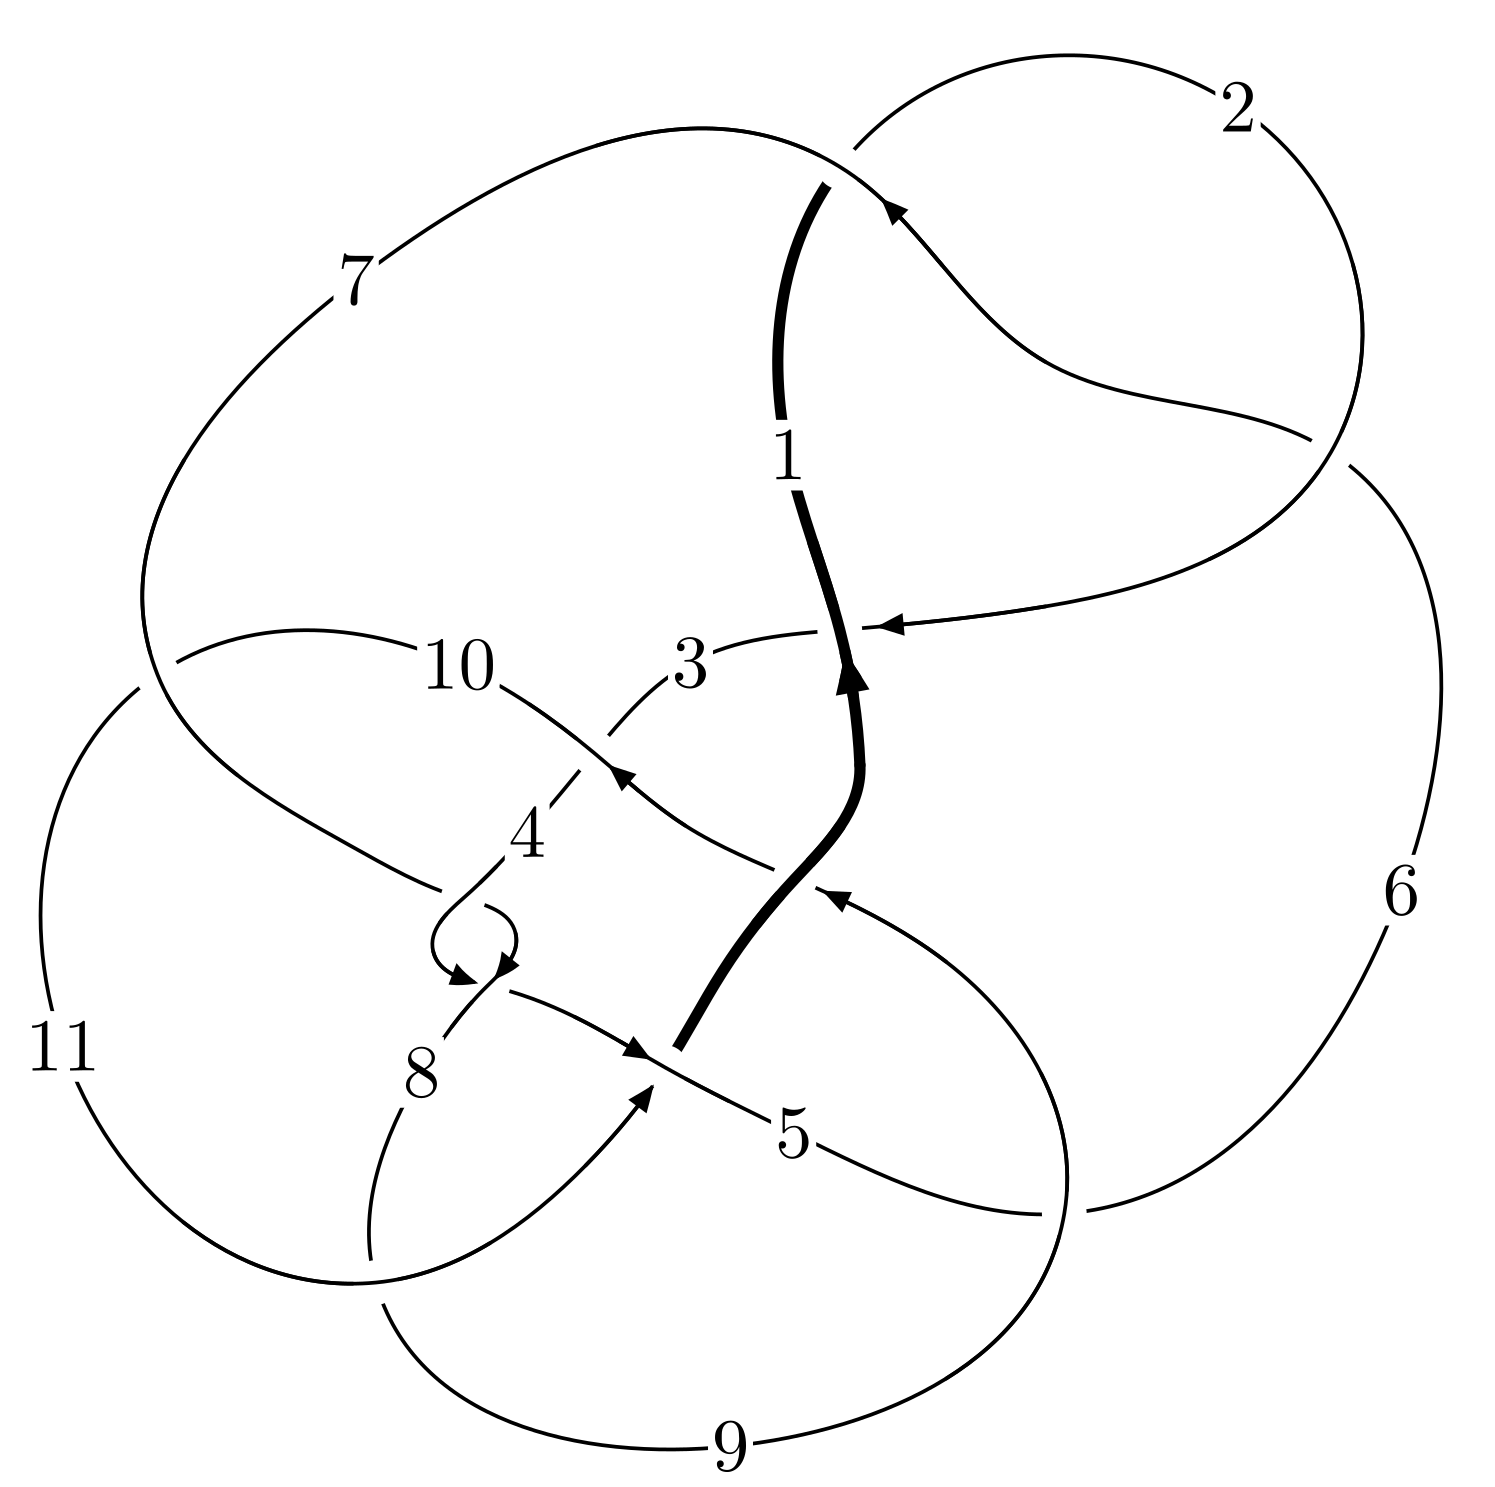
\includegraphics[width=112pt]{../../../GIT/diagram.site/Diagrams/png/744_11n_128.png}\\
\ \ \ A knot diagram\footnotemark}&
\allowdisplaybreaks
\textbf{Linearized knot diagam} \\
\cline{2-2}
 &
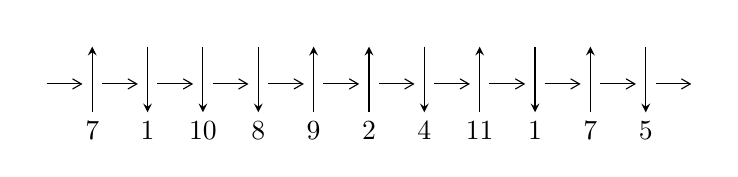
\begin{tikzpicture}[x=20pt, y=17pt]
	% nodes
	\node (C0) at (0, 0) {};
	\node (C1) at (1, 0) {};
	\node (C1U) at (1, +1) {};
	\node (C1D) at (1, -1) {7};

	\node (C2) at (2, 0) {};
	\node (C2U) at (2, +1) {};
	\node (C2D) at (2, -1) {1};

	\node (C3) at (3, 0) {};
	\node (C3U) at (3, +1) {};
	\node (C3D) at (3, -1) {10};

	\node (C4) at (4, 0) {};
	\node (C4U) at (4, +1) {};
	\node (C4D) at (4, -1) {8};

	\node (C5) at (5, 0) {};
	\node (C5U) at (5, +1) {};
	\node (C5D) at (5, -1) {9};

	\node (C6) at (6, 0) {};
	\node (C6U) at (6, +1) {};
	\node (C6D) at (6, -1) {2};

	\node (C7) at (7, 0) {};
	\node (C7U) at (7, +1) {};
	\node (C7D) at (7, -1) {4};

	\node (C8) at (8, 0) {};
	\node (C8U) at (8, +1) {};
	\node (C8D) at (8, -1) {11};

	\node (C9) at (9, 0) {};
	\node (C9U) at (9, +1) {};
	\node (C9D) at (9, -1) {1};

	\node (C10) at (10, 0) {};
	\node (C10U) at (10, +1) {};
	\node (C10D) at (10, -1) {7};

	\node (C11) at (11, 0) {};
	\node (C11U) at (11, +1) {};
	\node (C11D) at (11, -1) {5};
	\node (C12) at (12, 0) {};

	% arrows
	\draw[->,>={angle 60}]
	(C0) edge (C1) (C1) edge (C2) (C2) edge (C3) (C3) edge (C4) (C4) edge (C5) (C5) edge (C6) (C6) edge (C7) (C7) edge (C8) (C8) edge (C9) (C9) edge (C10) (C10) edge (C11) (C11) edge (C12) ;	\draw[->,>=stealth]
	(C1D) edge (C1U) (C2U) edge (C2D) (C3U) edge (C3D) (C4U) edge (C4D) (C5D) edge (C5U) (C6D) edge (C6U) (C7U) edge (C7D) (C8D) edge (C8U) (C9U) edge (C9D) (C10D) edge (C10U) (C11U) edge (C11D) ;
	\end{tikzpicture} \\
\hhline{~~} \\& 
\textbf{Solving Sequence} \\ \cline{2-2} 
 &
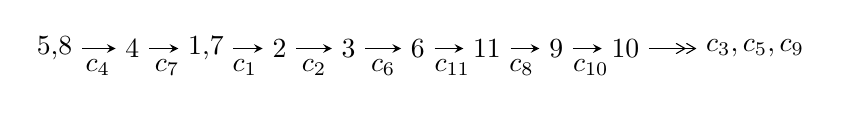
\begin{tikzpicture}[x=25pt, y=7pt]
	% node
	\node (A0) at (-1/8, 0) {5,8};
	\node (A1) at (1, 0) {4};
	\node (A2) at (33/16, 0) {1,7};
	\node (A3) at (25/8, 0) {2};
	\node (A4) at (33/8, 0) {3};
	\node (A5) at (41/8, 0) {6};
	\node (A6) at (49/8, 0) {11};
	\node (A7) at (57/8, 0) {9};
	\node (A8) at (65/8, 0) {10};
	\node (C1) at (1/2, -1) {$c_{4}$};
	\node (C2) at (3/2, -1) {$c_{7}$};
	\node (C3) at (21/8, -1) {$c_{1}$};
	\node (C4) at (29/8, -1) {$c_{2}$};
	\node (C5) at (37/8, -1) {$c_{6}$};
	\node (C6) at (45/8, -1) {$c_{11}$};
	\node (C7) at (53/8, -1) {$c_{8}$};
	\node (C8) at (61/8, -1) {$c_{10}$};
	\node (A9) at (10, 0) {$c_{3},c_{5},c_{9}$};

	% edge
	\draw[->,>=stealth]	
	(A0) edge (A1) (A1) edge (A2) (A2) edge (A3) (A3) edge (A4) (A4) edge (A5) (A5) edge (A6) (A6) edge (A7) (A7) edge (A8) ;
	\draw[->>,>={angle 60}]	
	(A8) edge (A9);
\end{tikzpicture} \\ 

\end{tabular} \\

\footnotetext{
The image of knot diagram is generated by the software ``\textbf{Draw programme}" developed by Andrew Bartholomew(\url{http://www.layer8.co.uk/maths/draw/index.htm\#Running-draw}), where we modified some parts for our purpose(\url{https://github.com/CATsTAILs/LinksPainter}).
}\phantom \\ \newline 
\centering \textbf{Ideals for irreducible components\footnotemark of $X_{\text{par}}$} 
 
\begin{align*}
I^u_{1}&=\langle 
9.89687\times10^{16} u^{31}-1.71588\times10^{17} u^{30}+\cdots+5.00890\times10^{17} b-1.23096\times10^{18},\\
\phantom{I^u_{1}}&\phantom{= \langle  }2.33797\times10^{16} u^{31}+9.75324\times10^{17} u^{30}+\cdots+5.00890\times10^{17} a+3.69251\times10^{18},\;u^{32}- u^{31}+\cdots-12 u+1\rangle \\
I^u_{2}&=\langle 
-7 u^{10}-4 u^9+22 u^8-29 u^6+17 u^5+14 u^4-7 u^3+3 u^2+13 b-9 u-1,\\
\phantom{I^u_{2}}&\phantom{= \langle  }17 u^{10}+6 u^9-59 u^8+26 u^7+63 u^6-71 u^5+18 u^4+17 u^3-50 u^2+39 a+59 u-31,\\
\phantom{I^u_{2}}&\phantom{= \langle  }u^{11}-4 u^9+u^8+6 u^7-4 u^6-3 u^5+4 u^4- u^3+u^2+u-3\rangle \\
\\
\end{align*}
\raggedright * 2 irreducible components of $\dim_{\mathbb{C}}=0$, with total 43 representations.\\
\footnotetext{All coefficients of polynomials are rational numbers. But the coefficients are sometimes approximated in decimal forms when there is not enough margin.}
\newpage
\renewcommand{\arraystretch}{1}
\centering \section*{I. $I^u_{1}= \langle 9.90\times10^{16} u^{31}-1.72\times10^{17} u^{30}+\cdots+5.01\times10^{17} b-1.23\times10^{18},\;2.34\times10^{16} u^{31}+9.75\times10^{17} u^{30}+\cdots+5.01\times10^{17} a+3.69\times10^{18},\;u^{32}- u^{31}+\cdots-12 u+1 \rangle$}
\flushleft \textbf{(i) Arc colorings}\\
\begin{tabular}{m{7pt} m{180pt} m{7pt} m{180pt} }
\flushright $a_{5}=$&$\begin{pmatrix}1\\0\end{pmatrix}$ \\
\flushright $a_{8}=$&$\begin{pmatrix}0\\u\end{pmatrix}$ \\
\flushright $a_{4}=$&$\begin{pmatrix}1\\- u^2\end{pmatrix}$ \\
\flushright $a_{1}=$&$\begin{pmatrix}-0.0466763 u^{31}-1.94718 u^{30}+\cdots+64.5722 u-7.37190\\-0.197586 u^{31}+0.342566 u^{30}+\cdots-13.4573 u+2.45755\end{pmatrix}$ \\
\flushright $a_{7}=$&$\begin{pmatrix}u\\- u^3+u\end{pmatrix}$ \\
\flushright $a_{2}=$&$\begin{pmatrix}-0.590773 u^{31}-1.76202 u^{30}+\cdots+59.4915 u-6.72272\\-0.199663 u^{31}+0.213550 u^{30}+\cdots-14.7748 u+2.74780\end{pmatrix}$ \\
\flushright $a_{3}=$&$\begin{pmatrix}4.28025 u^{31}+0.484730 u^{30}+\cdots+54.0490 u-3.93592\\-2.66133 u^{31}-0.797429 u^{30}+\cdots-30.9601 u+3.50979\end{pmatrix}$ \\
\flushright $a_{6}=$&$\begin{pmatrix}-1.93811 u^{31}-0.942980 u^{30}+\cdots-25.2538 u+6.08360\\1.07477 u^{31}+0.752123 u^{30}+\cdots+0.523274 u+0.239711\end{pmatrix}$ \\
\flushright $a_{11}=$&$\begin{pmatrix}-0.244262 u^{31}-1.60461 u^{30}+\cdots+51.1148 u-4.91435\\-0.197586 u^{31}+0.342566 u^{30}+\cdots-13.4573 u+2.45755\end{pmatrix}$ \\
\flushright $a_{9}=$&$\begin{pmatrix}3.39545 u^{31}-1.12542 u^{30}+\cdots+65.7600 u-9.37715\\0.771918 u^{31}-0.0178954 u^{30}+\cdots+15.0150 u-1.00246\end{pmatrix}$ \\
\flushright $a_{10}=$&$\begin{pmatrix}0.828985 u^{31}-1.68179 u^{30}+\cdots+60.1743 u-5.88389\\-0.589274 u^{31}+0.367301 u^{30}+\cdots-15.2775 u+2.48408\end{pmatrix}$\\ \flushright $a_{10}=$&$\begin{pmatrix}0.828985 u^{31}-1.68179 u^{30}+\cdots+60.1743 u-5.88389\\-0.589274 u^{31}+0.367301 u^{30}+\cdots-15.2775 u+2.48408\end{pmatrix}$\\&\end{tabular}
\flushleft \textbf{(ii) Obstruction class $= -1$}\\~\\
\flushleft \textbf{(iii) Cusp Shapes $= -\frac{1330608910123401616}{500890495867945381} u^{31}+\frac{476105635560304404}{500890495867945381} u^{30}+\cdots-\frac{27689584720904947212}{500890495867945381} u+\frac{917819854187100340}{500890495867945381}$}\\~\\
\newpage\renewcommand{\arraystretch}{1}
\flushleft \textbf{(iv) u-Polynomials at the component}\newline \\
\begin{tabular}{m{50pt}|m{274pt}}
Crossings & \hspace{64pt}u-Polynomials at each crossing \\
\hline $$\begin{aligned}c_{1},c_{6}\end{aligned}$$&$\begin{aligned}
&u^{32}+u^{31}+\cdots-20 u+1
\end{aligned}$\\
\hline $$\begin{aligned}c_{2}\end{aligned}$$&$\begin{aligned}
&u^{32}+47 u^{31}+\cdots-80 u+1
\end{aligned}$\\
\hline $$\begin{aligned}c_{3}\end{aligned}$$&$\begin{aligned}
&u^{32}-28 u^{30}+\cdots+154 u+43
\end{aligned}$\\
\hline $$\begin{aligned}c_{4},c_{7}\end{aligned}$$&$\begin{aligned}
&u^{32}+u^{31}+\cdots+12 u+1
\end{aligned}$\\
\hline $$\begin{aligned}c_{5}\end{aligned}$$&$\begin{aligned}
&u^{32}-2 u^{31}+\cdots+2606 u+1291
\end{aligned}$\\
\hline $$\begin{aligned}c_{8}\end{aligned}$$&$\begin{aligned}
&u^{32}+9 u^{31}+\cdots+26 u+1
\end{aligned}$\\
\hline $$\begin{aligned}c_{9}\end{aligned}$$&$\begin{aligned}
&u^{32}+4 u^{31}+\cdots-2696 u+589
\end{aligned}$\\
\hline $$\begin{aligned}c_{10}\end{aligned}$$&$\begin{aligned}
&u^{32}-3 u^{31}+\cdots-7138 u+3929
\end{aligned}$\\
\hline $$\begin{aligned}c_{11}\end{aligned}$$&$\begin{aligned}
&u^{32}+2 u^{31}+\cdots+34 u+19
\end{aligned}$\\
\hline
\end{tabular}\\~\\
\newpage\renewcommand{\arraystretch}{1}
\flushleft \textbf{(v) Riley Polynomials at the component}\newline \\
\begin{tabular}{m{50pt}|m{274pt}}
Crossings & \hspace{64pt}Riley Polynomials at each crossing \\
\hline $$\begin{aligned}c_{1},c_{6}\end{aligned}$$&$\begin{aligned}
&y^{32}+47 y^{31}+\cdots-80 y+1
\end{aligned}$\\
\hline $$\begin{aligned}c_{2}\end{aligned}$$&$\begin{aligned}
&y^{32}-117 y^{31}+\cdots+5428 y+1
\end{aligned}$\\
\hline $$\begin{aligned}c_{3}\end{aligned}$$&$\begin{aligned}
&y^{32}-56 y^{31}+\cdots+323982 y+1849
\end{aligned}$\\
\hline $$\begin{aligned}c_{4},c_{7}\end{aligned}$$&$\begin{aligned}
&y^{32}-25 y^{31}+\cdots-34 y+1
\end{aligned}$\\
\hline $$\begin{aligned}c_{5}\end{aligned}$$&$\begin{aligned}
&y^{32}+24 y^{31}+\cdots+12176136 y+1666681
\end{aligned}$\\
\hline $$\begin{aligned}c_{8}\end{aligned}$$&$\begin{aligned}
&y^{32}+9 y^{31}+\cdots-248 y+1
\end{aligned}$\\
\hline $$\begin{aligned}c_{9}\end{aligned}$$&$\begin{aligned}
&y^{32}-62 y^{31}+\cdots+1792760 y+346921
\end{aligned}$\\
\hline $$\begin{aligned}c_{10}\end{aligned}$$&$\begin{aligned}
&y^{32}+37 y^{31}+\cdots+205149034 y+15437041
\end{aligned}$\\
\hline $$\begin{aligned}c_{11}\end{aligned}$$&$\begin{aligned}
&y^{32}-10 y^{31}+\cdots-3322 y+361
\end{aligned}$\\
\hline
\end{tabular}\\~\\
\newpage\flushleft \textbf{(vi) Complex Volumes and Cusp Shapes}
$$\begin{array}{c|c|c}  
\text{Solutions to }I^u_{1}& \I (\text{vol} + \sqrt{-1}CS) & \text{Cusp shape}\\
 \hline 
\begin{aligned}
u &= \phantom{-}0.138542 + 1.056330 I \\
a &= -0.033005 - 0.199971 I \\
b &= \phantom{-}0.733437 + 0.365394 I\end{aligned}
 & -1.06384 - 2.01989 I & -6.33778 + 3.45023 I \\ \hline\begin{aligned}
u &= \phantom{-}0.138542 - 1.056330 I \\
a &= -0.033005 + 0.199971 I \\
b &= \phantom{-}0.733437 - 0.365394 I\end{aligned}
 & -1.06384 + 2.01989 I & -6.33778 - 3.45023 I \\ \hline\begin{aligned}
u &= -0.170624 + 1.162780 I \\
a &= \phantom{-}0.216364 + 0.079987 I \\
b &= -1.081780 + 0.698388 I\end{aligned}
 & -11.45540 + 6.47625 I & -4.15728 - 4.26891 I \\ \hline\begin{aligned}
u &= -0.170624 - 1.162780 I \\
a &= \phantom{-}0.216364 - 0.079987 I \\
b &= -1.081780 - 0.698388 I\end{aligned}
 & -11.45540 - 6.47625 I & -4.15728 + 4.26891 I \\ \hline\begin{aligned}
u &= \phantom{-}1.195330 + 0.230217 I \\
a &= -1.244340 - 0.038979 I \\
b &= \phantom{-}1.100620 + 0.617950 I\end{aligned}
 & -2.64686 - 1.18437 I & -3.89291 + 0.66467 I \\ \hline\begin{aligned}
u &= \phantom{-}1.195330 - 0.230217 I \\
a &= -1.244340 + 0.038979 I \\
b &= \phantom{-}1.100620 - 0.617950 I\end{aligned}
 & -2.64686 + 1.18437 I & -3.89291 - 0.66467 I \\ \hline\begin{aligned}
u &= \phantom{-}1.219350 + 0.077393 I \\
a &= \phantom{-}1.81848 + 0.38645 I \\
b &= -1.37078 - 1.24326 I\end{aligned}
 & -4.27477 - 2.33689 I & -7.63645 + 2.31412 I \\ \hline\begin{aligned}
u &= \phantom{-}1.219350 - 0.077393 I \\
a &= \phantom{-}1.81848 - 0.38645 I \\
b &= -1.37078 + 1.24326 I\end{aligned}
 & -4.27477 + 2.33689 I & -7.63645 - 2.31412 I \\ \hline\begin{aligned}
u &= -1.223500 + 0.038660 I \\
a &= \phantom{-}1.51818 - 0.66151 I \\
b &= -0.815453 - 0.142941 I\end{aligned}
 & -5.17336 + 1.79108 I & -9.36406 - 4.29945 I \\ \hline\begin{aligned}
u &= -1.223500 - 0.038660 I \\
a &= \phantom{-}1.51818 + 0.66151 I \\
b &= -0.815453 + 0.142941 I\end{aligned}
 & -5.17336 - 1.79108 I & -9.36406 + 4.29945 I\\
 \hline 
 \end{array}$$\newpage$$\begin{array}{c|c|c}  
\text{Solutions to }I^u_{1}& \I (\text{vol} + \sqrt{-1}CS) & \text{Cusp shape}\\
 \hline 
\begin{aligned}
u &= \phantom{-}0.535771 + 0.550945 I \\
a &= -0.124257 - 0.519984 I \\
b &= \phantom{-}0.049461 + 0.604800 I\end{aligned}
 & -0.34099 - 1.52893 I & -0.59741 + 5.96300 I \\ \hline\begin{aligned}
u &= \phantom{-}0.535771 - 0.550945 I \\
a &= -0.124257 + 0.519984 I \\
b &= \phantom{-}0.049461 - 0.604800 I\end{aligned}
 & -0.34099 + 1.52893 I & -0.59741 - 5.96300 I \\ \hline\begin{aligned}
u &= -1.197230 + 0.303844 I \\
a &= -1.37383 - 0.46524 I \\
b &= \phantom{-}0.874051 - 0.767936 I\end{aligned}
 & -1.91400 + 4.83866 I & -2.54787 - 6.95016 I \\ \hline\begin{aligned}
u &= -1.197230 - 0.303844 I \\
a &= -1.37383 + 0.46524 I \\
b &= \phantom{-}0.874051 + 0.767936 I\end{aligned}
 & -1.91400 - 4.83866 I & -2.54787 + 6.95016 I \\ \hline\begin{aligned}
u &= \phantom{-}1.224970 + 0.159550 I \\
a &= -2.65656 - 0.99246 I \\
b &= \phantom{-}0.670400 + 0.174363 I\end{aligned}
 & -13.62100 - 1.88059 I & -11.51732 + 4.17618 I \\ \hline\begin{aligned}
u &= \phantom{-}1.224970 - 0.159550 I \\
a &= -2.65656 + 0.99246 I \\
b &= \phantom{-}0.670400 - 0.174363 I\end{aligned}
 & -13.62100 + 1.88059 I & -11.51732 - 4.17618 I \\ \hline\begin{aligned}
u &= -1.295740 + 0.161402 I \\
a &= -1.07414 - 1.17404 I \\
b &= \phantom{-}1.19979 + 1.83348 I\end{aligned}
 & -14.4931 + 2.6399 I & -9.17083 - 2.92028 I \\ \hline\begin{aligned}
u &= -1.295740 - 0.161402 I \\
a &= -1.07414 + 1.17404 I \\
b &= \phantom{-}1.19979 - 1.83348 I\end{aligned}
 & -14.4931 - 2.6399 I & -9.17083 + 2.92028 I \\ \hline\begin{aligned}
u &= -0.162858 + 0.639240 I \\
a &= -0.550882 - 0.448237 I \\
b &= -0.529074 - 0.422527 I\end{aligned}
 & \phantom{-}1.26710 - 1.27122 I & \phantom{-}4.54373 + 1.02158 I \\ \hline\begin{aligned}
u &= -0.162858 - 0.639240 I \\
a &= -0.550882 + 0.448237 I \\
b &= -0.529074 + 0.422527 I\end{aligned}
 & \phantom{-}1.26710 + 1.27122 I & \phantom{-}4.54373 - 1.02158 I\\
 \hline 
 \end{array}$$\newpage$$\begin{array}{c|c|c}  
\text{Solutions to }I^u_{1}& \I (\text{vol} + \sqrt{-1}CS) & \text{Cusp shape}\\
 \hline 
\begin{aligned}
u &= -1.36987 + 0.42119 I \\
a &= \phantom{-}1.53053 - 0.02391 I \\
b &= -1.37290 + 0.81577 I\end{aligned}
 & -5.87267 + 7.08941 I & -7.09677 - 5.04780 I \\ \hline\begin{aligned}
u &= -1.36987 - 0.42119 I \\
a &= \phantom{-}1.53053 + 0.02391 I \\
b &= -1.37290 - 0.81577 I\end{aligned}
 & -5.87267 - 7.08941 I & -7.09677 + 5.04780 I \\ \hline\begin{aligned}
u &= \phantom{-}1.34905 + 0.49788 I \\
a &= \phantom{-}0.892282 - 0.609676 I \\
b &= -0.839959 - 0.308002 I\end{aligned}
 & -5.07213 - 3.71163 I & -7.67058 + 3.05284 I \\ \hline\begin{aligned}
u &= \phantom{-}1.34905 - 0.49788 I \\
a &= \phantom{-}0.892282 + 0.609676 I \\
b &= -0.839959 + 0.308002 I\end{aligned}
 & -5.07213 + 3.71163 I & -7.67058 - 3.05284 I \\ \hline\begin{aligned}
u &= \phantom{-}0.082800 + 0.471723 I \\
a &= \phantom{-}2.20738 + 1.65765 I \\
b &= -0.762439 + 0.930035 I\end{aligned}
 & -10.18920 - 0.37972 I & -2.16269 - 0.17573 I \\ \hline\begin{aligned}
u &= \phantom{-}0.082800 - 0.471723 I \\
a &= \phantom{-}2.20738 - 1.65765 I \\
b &= -0.762439 - 0.930035 I\end{aligned}
 & -10.18920 + 0.37972 I & -2.16269 + 0.17573 I \\ \hline\begin{aligned}
u &= \phantom{-}1.44332 + 0.48895 I \\
a &= -1.65118 + 0.16077 I \\
b &= \phantom{-}1.38562 + 0.96493 I\end{aligned}
 & -16.5743 - 12.2619 I & -6.15908 + 5.48895 I \\ \hline\begin{aligned}
u &= \phantom{-}1.44332 - 0.48895 I \\
a &= -1.65118 - 0.16077 I \\
b &= \phantom{-}1.38562 - 0.96493 I\end{aligned}
 & -16.5743 + 12.2619 I & -6.15908 - 5.48895 I \\ \hline\begin{aligned}
u &= -1.43379 + 0.69251 I \\
a &= -0.605697 - 0.669783 I \\
b &= \phantom{-}1.042800 + 0.178645 I\end{aligned}
 & -15.2091 + 0.2793 I & -8.54524 + 0. I\phantom{ +0.000000I} \\ \hline\begin{aligned}
u &= -1.43379 - 0.69251 I \\
a &= -0.605697 + 0.669783 I \\
b &= \phantom{-}1.042800 - 0.178645 I\end{aligned}
 & -15.2091 - 0.2793 I & -8.54524 + 0. I\phantom{ +0.000000I}\\
 \hline 
 \end{array}$$\newpage$$\begin{array}{c|c|c}  
\text{Solutions to }I^u_{1}& \I (\text{vol} + \sqrt{-1}CS) & \text{Cusp shape}\\
 \hline 
\begin{aligned}
u &= \phantom{-}0.164476 + 0.076390 I \\
a &= \phantom{-}1.63068 + 3.68897 I \\
b &= \phantom{-}0.716191 - 0.638089 I\end{aligned}
 & -1.10961 + 1.48762 I & -5.18747 - 2.41383 I \\ \hline\begin{aligned}
u &= \phantom{-}0.164476 - 0.076390 I \\
a &= \phantom{-}1.63068 - 3.68897 I \\
b &= \phantom{-}0.716191 + 0.638089 I\end{aligned}
 & -1.10961 - 1.48762 I & -5.18747 + 2.41383 I\\
 \hline 
 \end{array}$$\newpage\newpage\renewcommand{\arraystretch}{1}
\centering \section*{II. $I^u_{2}= \langle -7 u^{10}-4 u^9+\cdots+13 b-1,\;17 u^{10}+6 u^9+\cdots+39 a-31,\;u^{11}-4 u^9+\cdots+u-3 \rangle$}
\flushleft \textbf{(i) Arc colorings}\\
\begin{tabular}{m{7pt} m{180pt} m{7pt} m{180pt} }
\flushright $a_{5}=$&$\begin{pmatrix}1\\0\end{pmatrix}$ \\
\flushright $a_{8}=$&$\begin{pmatrix}0\\u\end{pmatrix}$ \\
\flushright $a_{4}=$&$\begin{pmatrix}1\\- u^2\end{pmatrix}$ \\
\flushright $a_{1}=$&$\begin{pmatrix}-0.435897 u^{10}-0.153846 u^{9}+\cdots-1.51282 u+0.794872\\0.538462 u^{10}+0.307692 u^{9}+\cdots+0.692308 u+0.0769231\end{pmatrix}$ \\
\flushright $a_{7}=$&$\begin{pmatrix}u\\- u^3+u\end{pmatrix}$ \\
\flushright $a_{2}=$&$\begin{pmatrix}0.487179 u^{10}-0.769231 u^{9}+\cdots+1.10256 u-0.358974\\0.384615 u^{10}+0.0769231 u^{9}+\cdots-0.0769231 u+0.769231\end{pmatrix}$ \\
\flushright $a_{3}=$&$\begin{pmatrix}1.12821 u^{10}-1.30769 u^{9}+\cdots+4.97436 u-3.41026\\-0.153846 u^{10}+0.769231 u^{9}+\cdots-1.76923 u+2.69231\end{pmatrix}$ \\
\flushright $a_{6}=$&$\begin{pmatrix}-0.641026 u^{10}+0.538462 u^{9}+\cdots-1.87179 u+2.05128\\-0.461538 u^{10}+0.307692 u^{9}+\cdots-1.30769 u+1.07692\end{pmatrix}$ \\
\flushright $a_{11}=$&$\begin{pmatrix}0.102564 u^{10}+0.153846 u^{9}+\cdots-0.820513 u+0.871795\\0.538462 u^{10}+0.307692 u^{9}+\cdots+0.692308 u+0.0769231\end{pmatrix}$ \\
\flushright $a_{9}=$&$\begin{pmatrix}-0.205128 u^{10}+0.692308 u^{9}+\cdots-0.358974 u+0.256410\\-0.461538 u^{10}+0.307692 u^{9}+\cdots-0.307692 u+0.0769231\end{pmatrix}$ \\
\flushright $a_{10}=$&$\begin{pmatrix}-0.897436 u^{10}+0.153846 u^{9}+\cdots-2.82051 u+0.871795\\0.538462 u^{10}+0.307692 u^{9}+\cdots+1.69231 u+0.0769231\end{pmatrix}$\\ \flushright $a_{10}=$&$\begin{pmatrix}-0.897436 u^{10}+0.153846 u^{9}+\cdots-2.82051 u+0.871795\\0.538462 u^{10}+0.307692 u^{9}+\cdots+1.69231 u+0.0769231\end{pmatrix}$\\&\end{tabular}
\flushleft \textbf{(ii) Obstruction class $= 1$}\\~\\
\flushleft \textbf{(iii) Cusp Shapes $= -\frac{25}{13} u^{10}-\frac{5}{13} u^9+\frac{73}{13} u^8- u^7-\frac{85}{13} u^6+\frac{57}{13} u^5+\frac{63}{13} u^4-\frac{38}{13} u^3-\frac{32}{13} u^2-\frac{8}{13} u-\frac{63}{13}$}\\~\\
\newpage\renewcommand{\arraystretch}{1}
\flushleft \textbf{(iv) u-Polynomials at the component}\newline \\
\begin{tabular}{m{50pt}|m{274pt}}
Crossings & \hspace{64pt}u-Polynomials at each crossing \\
\hline $$\begin{aligned}c_{1}\end{aligned}$$&$\begin{aligned}
&u^{11}+6 u^9+13 u^7+15 u^5+u^4+9 u^3+2 u^2+3 u+1
\end{aligned}$\\
\hline $$\begin{aligned}c_{2}\end{aligned}$$&$\begin{aligned}
&u^{11}+12 u^{10}+\cdots+5 u-1
\end{aligned}$\\
\hline $$\begin{aligned}c_{3}\end{aligned}$$&$\begin{aligned}
&u^{11}- u^{10}-3 u^9-3 u^8+u^7+7 u^6+12 u^5+15 u^4+11 u^3+7 u^2+3 u+1
\end{aligned}$\\
\hline $$\begin{aligned}c_{4}\end{aligned}$$&$\begin{aligned}
&u^{11}-4 u^9+u^8+6 u^7-4 u^6-3 u^5+4 u^4- u^3+u^2+u-3
\end{aligned}$\\
\hline $$\begin{aligned}c_{5}\end{aligned}$$&$\begin{aligned}
&u^{11}- u^{10}+u^9- u^8+4 u^7+u^5-4 u^4+2 u^3+u-1
\end{aligned}$\\
\hline $$\begin{aligned}c_{6}\end{aligned}$$&$\begin{aligned}
&u^{11}+6 u^9+13 u^7+15 u^5- u^4+9 u^3-2 u^2+3 u-1
\end{aligned}$\\
\hline $$\begin{aligned}c_{7}\end{aligned}$$&$\begin{aligned}
&u^{11}-4 u^9- u^8+6 u^7+4 u^6-3 u^5-4 u^4- u^3- u^2+u+3
\end{aligned}$\\
\hline $$\begin{aligned}c_{8}\end{aligned}$$&$\begin{aligned}
&u^{11}+2 u^{10}+u^9-4 u^8-6 u^7-2 u^6+9 u^5+13 u^4+9 u^3+2 u^2- u-1
\end{aligned}$\\
\hline $$\begin{aligned}c_{9}\end{aligned}$$&$\begin{aligned}
&u^{11}-9 u^{10}+\cdots+17 u-3
\end{aligned}$\\
\hline $$\begin{aligned}c_{10}\end{aligned}$$&$\begin{aligned}
&u^{11}+2 u^{10}+5 u^9+4 u^8+u^7- u^6-6 u^5+4 u^4-2 u^3+3 u^2-3 u+1
\end{aligned}$\\
\hline $$\begin{aligned}c_{11}\end{aligned}$$&$\begin{aligned}
&u^{11}+u^{10}+2 u^8+4 u^7+u^6+4 u^4+u^3+u^2+u+1
\end{aligned}$\\
\hline
\end{tabular}\\~\\
\newpage\renewcommand{\arraystretch}{1}
\flushleft \textbf{(v) Riley Polynomials at the component}\newline \\
\begin{tabular}{m{50pt}|m{274pt}}
Crossings & \hspace{64pt}Riley Polynomials at each crossing \\
\hline $$\begin{aligned}c_{1},c_{6}\end{aligned}$$&$\begin{aligned}
&y^{11}+12 y^{10}+\cdots+5 y-1
\end{aligned}$\\
\hline $$\begin{aligned}c_{2}\end{aligned}$$&$\begin{aligned}
&y^{11}-20 y^{10}+\cdots+121 y-1
\end{aligned}$\\
\hline $$\begin{aligned}c_{3}\end{aligned}$$&$\begin{aligned}
&y^{11}-7 y^{10}+\cdots-5 y-1
\end{aligned}$\\
\hline $$\begin{aligned}c_{4},c_{7}\end{aligned}$$&$\begin{aligned}
&y^{11}-8 y^{10}+\cdots+7 y-9
\end{aligned}$\\
\hline $$\begin{aligned}c_{5}\end{aligned}$$&$\begin{aligned}
&y^{11}+y^{10}+7 y^9+9 y^8+14 y^7+6 y^6+17 y^5-6 y^4+6 y^3-4 y^2+y-1
\end{aligned}$\\
\hline $$\begin{aligned}c_{8}\end{aligned}$$&$\begin{aligned}
&y^{11}-2 y^{10}+5 y^9-2 y^8+4 y^7+43 y^5+5 y^4+7 y^3+4 y^2+5 y-1
\end{aligned}$\\
\hline $$\begin{aligned}c_{9}\end{aligned}$$&$\begin{aligned}
&y^{11}-9 y^{10}+\cdots-35 y-9
\end{aligned}$\\
\hline $$\begin{aligned}c_{10}\end{aligned}$$&$\begin{aligned}
&y^{11}+6 y^{10}+11 y^9-14 y^8-71 y^7-83 y^6-18 y^5+18 y^3-5 y^2+3 y-1
\end{aligned}$\\
\hline $$\begin{aligned}c_{11}\end{aligned}$$&$\begin{aligned}
&y^{11}- y^{10}+4 y^9-6 y^8+6 y^7-17 y^6-6 y^5-14 y^4-9 y^3-7 y^2- y-1
\end{aligned}$\\
\hline
\end{tabular}\\~\\
\newpage\flushleft \textbf{(vi) Complex Volumes and Cusp Shapes}
$$\begin{array}{c|c|c}  
\text{Solutions to }I^u_{2}& \I (\text{vol} + \sqrt{-1}CS) & \text{Cusp shape}\\
 \hline 
\begin{aligned}
u &= \phantom{-}0.704223 + 0.799205 I \\
a &= \phantom{-}0.198244 + 0.688371 I \\
b &= \phantom{-}0.482497 - 0.432213 I\end{aligned}
 & -0.834177 - 0.664427 I & -5.62999 - 1.84817 I \\ \hline\begin{aligned}
u &= \phantom{-}0.704223 - 0.799205 I \\
a &= \phantom{-}0.198244 - 0.688371 I \\
b &= \phantom{-}0.482497 + 0.432213 I\end{aligned}
 & -0.834177 + 0.664427 I & -5.62999 + 1.84817 I \\ \hline\begin{aligned}
u &= -1.113080 + 0.252147 I \\
a &= \phantom{-}1.50946 + 0.63887 I \\
b &= -0.266277 - 0.765184 I\end{aligned}
 & -12.65170 + 1.14869 I & -5.06516 + 0.05051 I \\ \hline\begin{aligned}
u &= -1.113080 - 0.252147 I \\
a &= \phantom{-}1.50946 - 0.63887 I \\
b &= -0.266277 + 0.765184 I\end{aligned}
 & -12.65170 - 1.14869 I & -5.06516 - 0.05051 I \\ \hline\begin{aligned}
u &= \phantom{-}1.130350 + 0.302780 I \\
a &= \phantom{-}0.836611 + 0.061028 I \\
b &= -0.722191 - 1.091390 I\end{aligned}
 & -2.43632 - 3.36377 I & -4.69391 + 3.63598 I \\ \hline\begin{aligned}
u &= \phantom{-}1.130350 - 0.302780 I \\
a &= \phantom{-}0.836611 - 0.061028 I \\
b &= -0.722191 + 1.091390 I\end{aligned}
 & -2.43632 + 3.36377 I & -4.69391 - 3.63598 I \\ \hline\begin{aligned}
u &= -0.064226 + 0.786482 I \\
a &= \phantom{-}0.158980 - 0.213232 I \\
b &= -0.735500 - 0.606796 I\end{aligned}
 & \phantom{-}0.44585 - 2.19055 I & -0.27735 + 4.50255 I \\ \hline\begin{aligned}
u &= -0.064226 - 0.786482 I \\
a &= \phantom{-}0.158980 + 0.213232 I \\
b &= -0.735500 + 0.606796 I\end{aligned}
 & \phantom{-}0.44585 + 2.19055 I & -0.27735 - 4.50255 I \\ \hline\begin{aligned}
u &= \phantom{-}1.29327\phantom{ +0.000000I} \\
a &= -1.68071\phantom{ +0.000000I} \\
b &= \phantom{-}1.36323\phantom{ +0.000000I}\end{aligned}
 & -4.68995\phantom{ +0.000000I} & -8.42500\phantom{ +0.000000I} \\ \hline\begin{aligned}
u &= -1.303900 + 0.374956 I \\
a &= -1.69628 - 0.11240 I \\
b &= \phantom{-}1.059850 - 0.766199 I\end{aligned}
 & -3.56282 + 6.44913 I & -4.62110 - 5.90724 I\\
 \hline 
 \end{array}$$\newpage$$\begin{array}{c|c|c}  
\text{Solutions to }I^u_{2}& \I (\text{vol} + \sqrt{-1}CS) & \text{Cusp shape}\\
 \hline 
\begin{aligned}
u &= -1.303900 - 0.374956 I \\
a &= -1.69628 + 0.11240 I \\
b &= \phantom{-}1.059850 + 0.766199 I\end{aligned}
 & -3.56282 - 6.44913 I & -4.62110 + 5.90724 I\\
 \hline 
 \end{array}$$\newpage
\newpage\renewcommand{\arraystretch}{1}
\centering \section*{ III. u-Polynomials}
\begin{tabular}{m{50pt}|m{274pt}}
Crossings & \hspace{64pt}u-Polynomials at each crossing \\
\hline $$\begin{aligned}c_{1}\end{aligned}$$&$\begin{aligned}
&(u^{11}+6 u^9+13 u^7+15 u^5+u^4+9 u^3+2 u^2+3 u+1)\\
&\cdot(u^{32}+u^{31}+\cdots-20 u+1)
\end{aligned}$\\
\hline $$\begin{aligned}c_{2}\end{aligned}$$&$\begin{aligned}
&(u^{11}+12 u^{10}+\cdots+5 u-1)(u^{32}+47 u^{31}+\cdots-80 u+1)
\end{aligned}$\\
\hline $$\begin{aligned}c_{3}\end{aligned}$$&$\begin{aligned}
&(u^{11}- u^{10}-3 u^9-3 u^8+u^7+7 u^6+12 u^5+15 u^4+11 u^3+7 u^2+3 u+1)\\
&\cdot(u^{32}-28 u^{30}+\cdots+154 u+43)
\end{aligned}$\\
\hline $$\begin{aligned}c_{4}\end{aligned}$$&$\begin{aligned}
&(u^{11}-4 u^9+u^8+6 u^7-4 u^6-3 u^5+4 u^4- u^3+u^2+u-3)\\
&\cdot(u^{32}+u^{31}+\cdots+12 u+1)
\end{aligned}$\\
\hline $$\begin{aligned}c_{5}\end{aligned}$$&$\begin{aligned}
&(u^{11}- u^{10}+u^9- u^8+4 u^7+u^5-4 u^4+2 u^3+u-1)\\
&\cdot(u^{32}-2 u^{31}+\cdots+2606 u+1291)
\end{aligned}$\\
\hline $$\begin{aligned}c_{6}\end{aligned}$$&$\begin{aligned}
&(u^{11}+6 u^9+13 u^7+15 u^5- u^4+9 u^3-2 u^2+3 u-1)\\
&\cdot(u^{32}+u^{31}+\cdots-20 u+1)
\end{aligned}$\\
\hline $$\begin{aligned}c_{7}\end{aligned}$$&$\begin{aligned}
&(u^{11}-4 u^9- u^8+6 u^7+4 u^6-3 u^5-4 u^4- u^3- u^2+u+3)\\
&\cdot(u^{32}+u^{31}+\cdots+12 u+1)
\end{aligned}$\\
\hline $$\begin{aligned}c_{8}\end{aligned}$$&$\begin{aligned}
&(u^{11}+2 u^{10}+u^9-4 u^8-6 u^7-2 u^6+9 u^5+13 u^4+9 u^3+2 u^2- u-1)\\
&\cdot(u^{32}+9 u^{31}+\cdots+26 u+1)
\end{aligned}$\\
\hline $$\begin{aligned}c_{9}\end{aligned}$$&$\begin{aligned}
&(u^{11}-9 u^{10}+\cdots+17 u-3)(u^{32}+4 u^{31}+\cdots-2696 u+589)
\end{aligned}$\\
\hline $$\begin{aligned}c_{10}\end{aligned}$$&$\begin{aligned}
&(u^{11}+2 u^{10}+5 u^9+4 u^8+u^7- u^6-6 u^5+4 u^4-2 u^3+3 u^2-3 u+1)\\
&\cdot(u^{32}-3 u^{31}+\cdots-7138 u+3929)
\end{aligned}$\\
\hline $$\begin{aligned}c_{11}\end{aligned}$$&$\begin{aligned}
&(u^{11}+u^{10}+2 u^8+4 u^7+u^6+4 u^4+u^3+u^2+u+1)\\
&\cdot(u^{32}+2 u^{31}+\cdots+34 u+19)
\end{aligned}$\\
\hline
\end{tabular}\newpage\renewcommand{\arraystretch}{1}
\centering \section*{ IV. Riley Polynomials}
\begin{tabular}{m{50pt}|m{274pt}}
Crossings & \hspace{64pt}Riley Polynomials at each crossing \\
\hline $$\begin{aligned}c_{1},c_{6}\end{aligned}$$&$\begin{aligned}
&(y^{11}+12 y^{10}+\cdots+5 y-1)(y^{32}+47 y^{31}+\cdots-80 y+1)
\end{aligned}$\\
\hline $$\begin{aligned}c_{2}\end{aligned}$$&$\begin{aligned}
&(y^{11}-20 y^{10}+\cdots+121 y-1)(y^{32}-117 y^{31}+\cdots+5428 y+1)
\end{aligned}$\\
\hline $$\begin{aligned}c_{3}\end{aligned}$$&$\begin{aligned}
&(y^{11}-7 y^{10}+\cdots-5 y-1)(y^{32}-56 y^{31}+\cdots+323982 y+1849)
\end{aligned}$\\
\hline $$\begin{aligned}c_{4},c_{7}\end{aligned}$$&$\begin{aligned}
&(y^{11}-8 y^{10}+\cdots+7 y-9)(y^{32}-25 y^{31}+\cdots-34 y+1)
\end{aligned}$\\
\hline $$\begin{aligned}c_{5}\end{aligned}$$&$\begin{aligned}
&(y^{11}+y^{10}+7 y^9+9 y^8+14 y^7+6 y^6+17 y^5-6 y^4+6 y^3-4 y^2+y-1)\\
&\cdot(y^{32}+24 y^{31}+\cdots+12176136 y+1666681)
\end{aligned}$\\
\hline $$\begin{aligned}c_{8}\end{aligned}$$&$\begin{aligned}
&(y^{11}-2 y^{10}+5 y^9-2 y^8+4 y^7+43 y^5+5 y^4+7 y^3+4 y^2+5 y-1)\\
&\cdot(y^{32}+9 y^{31}+\cdots-248 y+1)
\end{aligned}$\\
\hline $$\begin{aligned}c_{9}\end{aligned}$$&$\begin{aligned}
&(y^{11}-9 y^{10}+\cdots-35 y-9)(y^{32}-62 y^{31}+\cdots+1792760 y+346921)
\end{aligned}$\\
\hline $$\begin{aligned}c_{10}\end{aligned}$$&$\begin{aligned}
&(y^{11}+6 y^{10}+11 y^9-14 y^8-71 y^7-83 y^6-18 y^5+18 y^3-5 y^2+3 y-1)\\
&\cdot(y^{32}+37 y^{31}+\cdots+205149034 y+15437041)
\end{aligned}$\\
\hline $$\begin{aligned}c_{11}\end{aligned}$$&$\begin{aligned}
&(y^{11}- y^{10}+4 y^9-6 y^8+6 y^7-17 y^6-6 y^5-14 y^4-9 y^3-7 y^2- y-1)\\
&\cdot(y^{32}-10 y^{31}+\cdots-3322 y+361)
\end{aligned}$\\
\hline
\end{tabular}
\vskip 2pc
\end{document}